\begin{figure}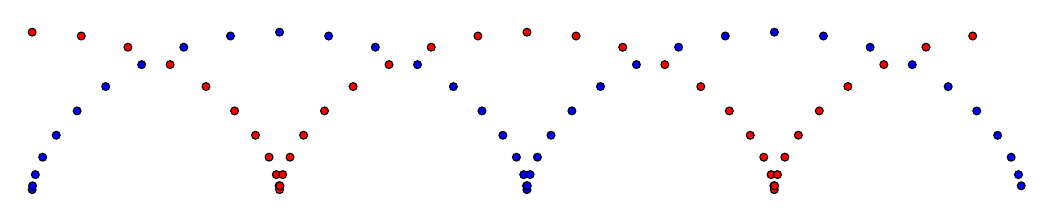
\begin{tikzpicture}[scale=1, rotate=0]

% two ornac of a photon  going through two cycloid cycle in red

%% red ornac
 \foreach \x in {0, 0.05,...,2}
  {
    \draw[black, fill=red] 
   ({((2*pi*\x + sin(2*pi*\x r)) },{1 + cos(2*pi*\x r) }) circle [radius=0.05];
  }


%% blue ornac
 \foreach \x in {0, 0.05,...,2}
  {
    \draw[black, fill=blue] 
   ({((2*pi*\x + sin((2*pi*\x -pi) r)) },{1 + cos((2*pi*\x -pi) r) }) circle [radius=0.05];
  }

\end{tikzpicture}
\caption{Two ornac of a photon  going through two cycloid cycle in red and blue
\label{fig:two_ornac_cycloid}}
\end{figure}
